% Requires \usepackage{graphicx}. Use figure* for two-column layouts.
\begin{figure*}[t]
  \centering
  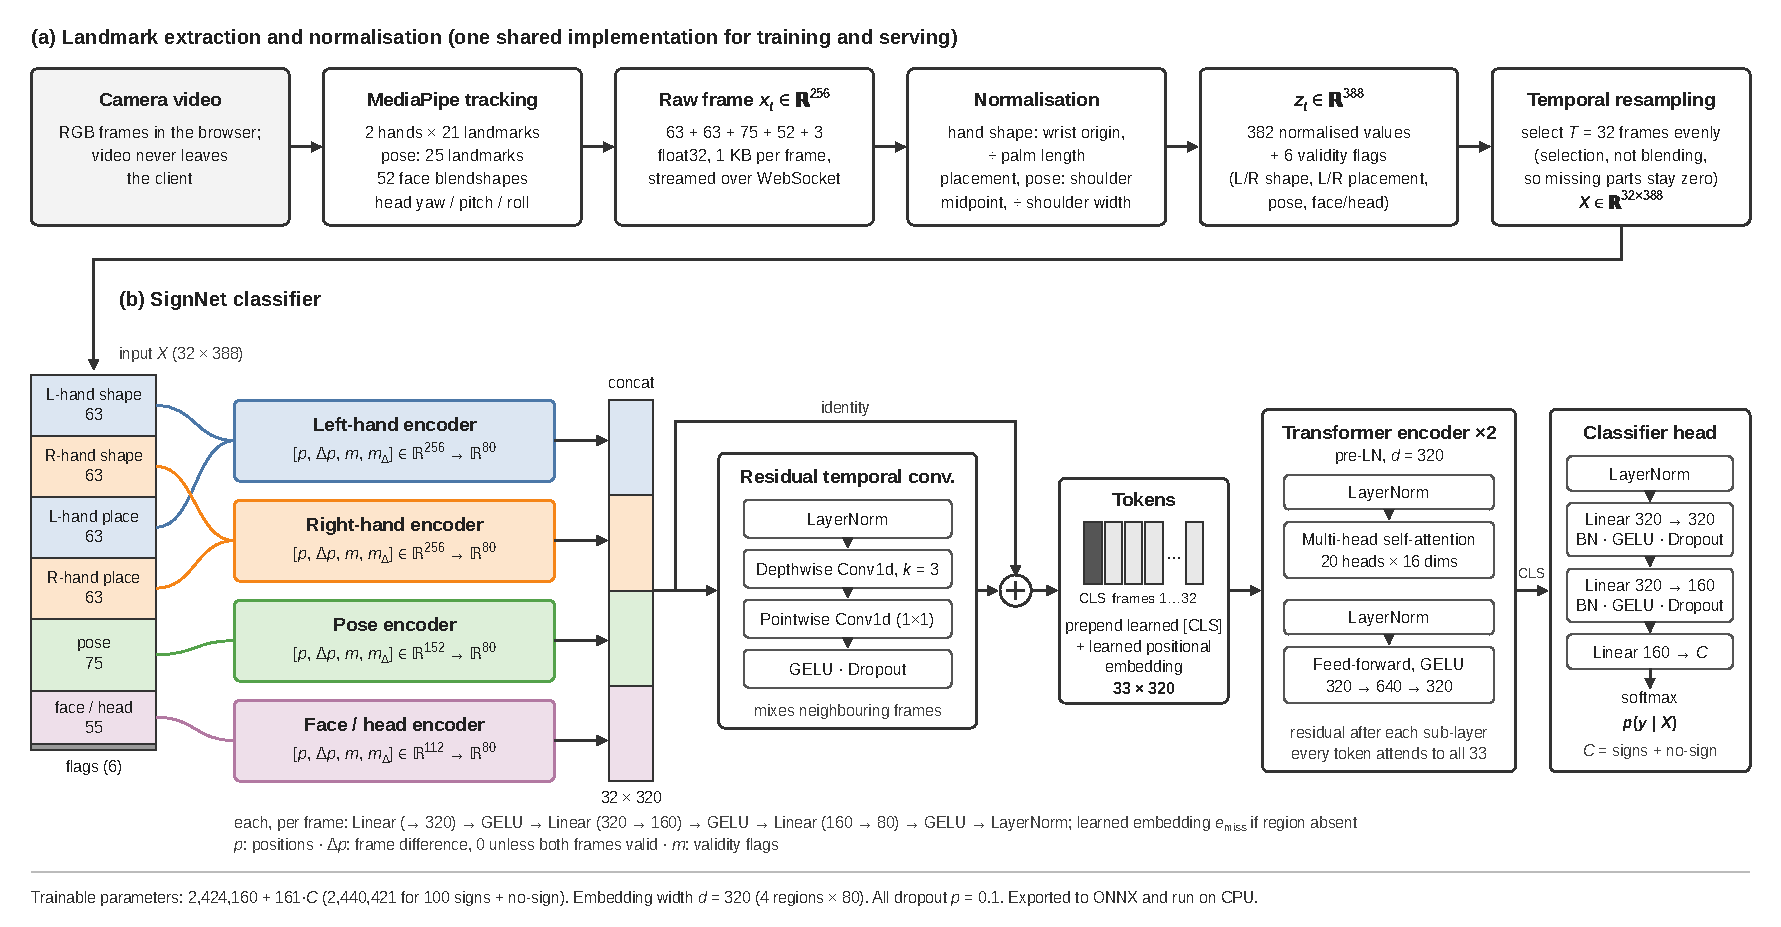
\includegraphics[width=\textwidth]{figures/fig1_architecture.pdf}
  \caption{System and model architecture. (a) MediaPipe landmarks are extracted in the
  browser; each frame is normalised (hand shape relative to the wrist and palm length;
  hand placement and pose relative to the shoulder midpoint and shoulder width), augmented
  with six validity flags, and resampled to $T{=}32$ frames, giving $X \in \mathbb{R}^{32\times388}$.
  (b) SignNet encodes four anatomical regions separately from positions, masked frame
  differences and validity flags (80 dimensions each, with a learned embedding for absent
  regions), mixes neighbouring frames with a residual depthwise-separable temporal
  convolution, and classifies a learned [CLS] token after two pre-LN Transformer encoder
  layers. The output covers all signs plus a no-sign class.}
  \label{fig:architecture}
\end{figure*}

\begin{figure*}[t]
  \centering
  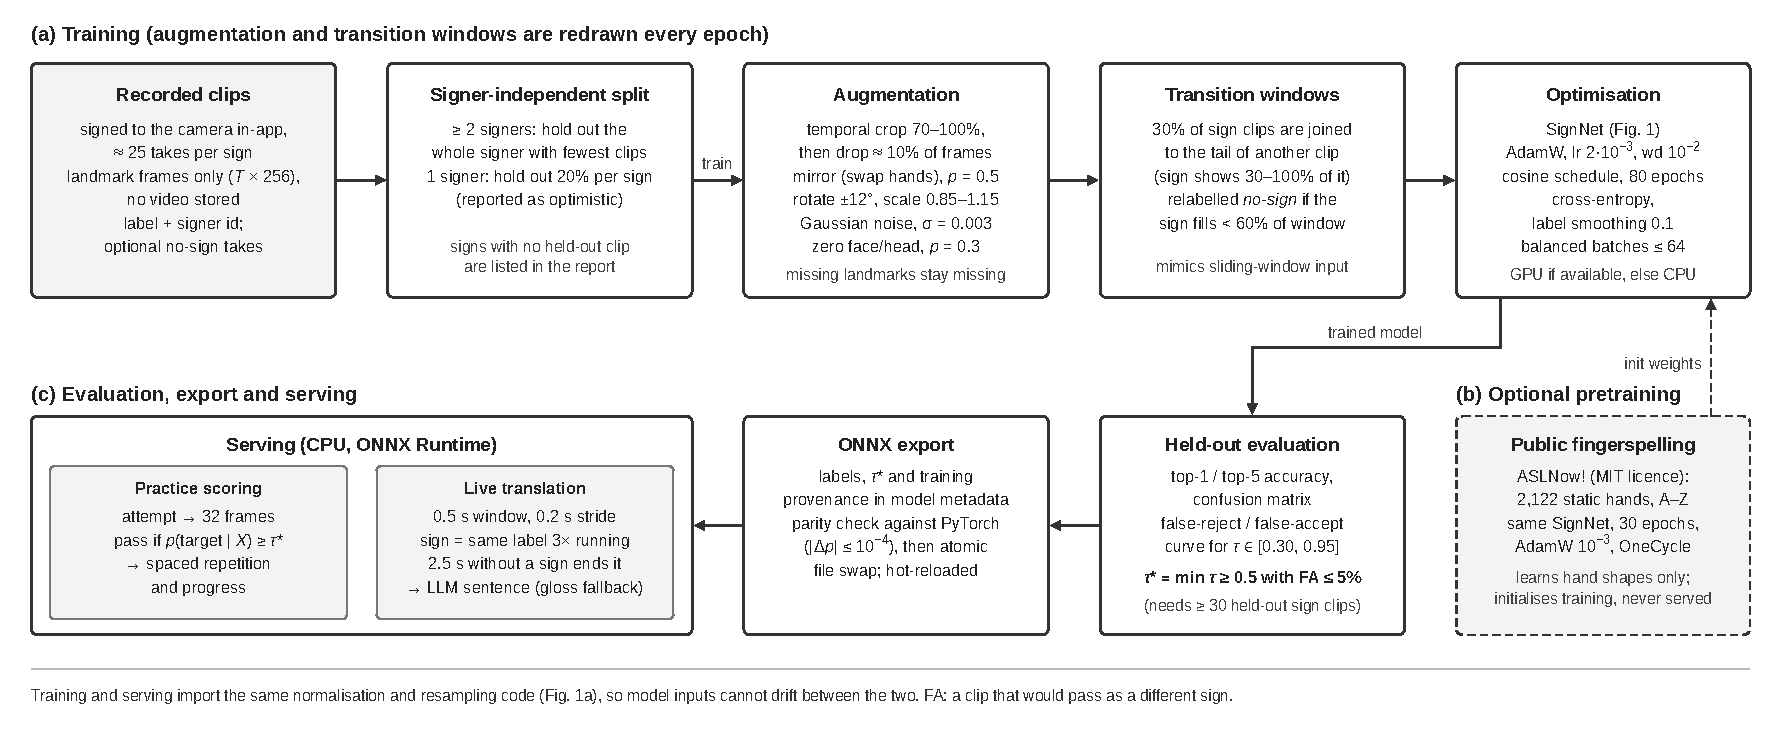
\includegraphics[width=\textwidth]{figures/fig2_training.pdf}
  \caption{Training and deployment pipeline. (a) Clips are split by signer, then augmented
  and mixed into transition windows afresh every epoch before optimisation. (b) Optional
  pretraining on public fingerspelling data initialises the weights. (c) The held-out set
  selects the pass threshold $\tau^*$ that keeps false accepts at or below 5\%; the model is
  exported to ONNX with a numerical parity check and served on CPU for practice scoring and
  sliding-window live translation.}
  \label{fig:training}
\end{figure*}
